\documentclass[12pt,a4paper]{article}
\usepackage[utf8]{inputenc}
\usepackage[portuguese]{babel}
\usepackage{geometry}
\usepackage{graphicx}
\usepackage{amsmath, amsfonts, amssymb}
\usepackage{listings}
\usepackage{xcolor}
\usepackage{booktabs}
\usepackage{longtable}
\usepackage{array}
\usepackage{hyperref}
\usepackage{fancyhdr}
\usepackage{titlesec}
\usepackage{enumitem}
\usepackage{setspace}     % Para espaçamento
\usepackage{lipsum}       % Texto de exemplo

% Configurações da página
\geometry{top=2.5cm, bottom=2.5cm, left=3cm, right=3cm}
\setstretch{1.5}  % Espaçamento entre linhas

% Cabeçalho e rodapé
\pagestyle{fancy}
\fancyhf{}
\fancyhead[L]{Data Lake Azure - Sistema de Saúde}
\fancyhead[R]{\thepage}
\renewcommand{\headrulewidth}{0.4pt}

% Estilo para código SQL
\lstdefinestyle{sqlstyle}{
    language=SQL,
    basicstyle=\footnotesize\ttfamily,
    keywordstyle=\color{blue},
    commentstyle=\color{gray},
    stringstyle=\color{red},
    showstringspaces=false,
    breaklines=true,
    frame=single,
    backgroundcolor=\color{gray!10},
    captionpos=b
}

% Títulos
\titleformat{\section}{\Large\bfseries}{\thesection}{1em}{}
\titleformat{\subsection}{\large\bfseries}{\thesubsection}{1em}{}

% CAPA
\begin{document}
\begin{titlepage}
    \centering
    
\includegraphics[width=0.15\textwidth]{logo_pucrs.png} % Logo da PUCRS, se desejar

    \vspace*{2cm}
    {\Large \textbf{PONTIFÍCIA UNIVERSIDADE CATÓLICA DO RIO GRANDE DO SUL}}\\[0.3cm]
    {\large \textbf{ESCOLA POLITÉCNICA}}\\[1.2cm]
    
    \vfill

    {\Huge \textbf{AZURE DATA LAKE}}\\[0.4cm]
    {\Large \textbf{Relatório Técnico Final}}\\[0.5cm]
    {\large \textit{Sistema Integrado de Informações de Saúde}}\\

    \vfill

    \begin{flushleft}
    \textbf{Autores:}
    \begin{itemize}[leftmargin=1.5cm]
        \item Bruna Marschner – Ciência de Dados e Inteligência Artificial
        \item Gustavo Filipi Lopes Machado – Ciência da Computação
        \item Lucas dos Santos Vizzotto – Ciência de Dados e Inteligência Artificial
    \end{itemize}

    \vspace{1cm}
    \textbf{Data de Entrega:} \today
    \end{flushleft}


\end{titlepage}
\newpage
\tableofcontents
\newpage

\section{IDENTIFICAÇÃO DO PROJETO}

\begin{itemize}[leftmargin=2cm]
    \item \textbf{Grupo de Recursos Azure:} grupo14 (grup014 no Azure)
    \item \textbf{Domínio da Aplicação:} Sistema de Saúde Pública
    \item \textbf{Fontes de Dados:} GERINT (Gestão de Regulação de Internações) + SINASC (Sistema de Informações sobre Nascidos Vivos)
\end{itemize}

\section{ESQUEMA CONCEITUAL DAS FONTES DE DADOS}

\subsection{Primeira Fonte - GERINT (Sistema de Regulação de Internações)}

\textbf{Classes Principais:}
\begin{itemize}
    \item \textbf{Paciente:} Dados demográficos dos pacientes
    \item \textbf{Solicitação de Internação:} Pedidos de internação hospitalar
    \item \textbf{Tipo de Leito:} Categorização dos leitos disponíveis
    \item \textbf{Diagnóstico:} Códigos CID e descrições
    \item \textbf{Estabelecimento de Saúde:} Hospitais e unidades de saúde
\end{itemize}

\subsection{Segunda Fonte - SINASC (Nascimentos)}

\textbf{Classes Principais:}
\begin{itemize}
    \item \textbf{Nascimento:} Registro principal do nascimento
    \item \textbf{Dados da Mãe:} Informações maternas (escolaridade, raça, ocupação)
    \item \textbf{Dados da Gestação:} Informações do período gestacional
    \item \textbf{Dados do Parto:} Detalhes sobre o processo de parto
\end{itemize}

\subsection{Relacionamento entre as Fontes}

\textbf{Chave de Ligação:} Código CID (Classificação Internacional de Doenças)

Anomalias congênitas registradas nos nascimentos podem gerar futuras solicitações de internação, permitindo análise epidemiológica integrada entre nascimentos e internações.

\section{PRIMEIRA FONTE DE DADOS - POSTGRESQL}

\subsection{Esquema Lógico Relacional}

\textbf{Tabelas Principais:}
\begin{enumerate}
    \item \textbf{pacientes} - Dados demográficos
    \item \textbf{solicitacoes\_internacao} - Pedidos de internação
    \item \textbf{tipos\_leito} - Tipos e categorias de leitos
    \item \textbf{diagnosticos} - Códigos CID
    \item \textbf{estabelecimentos\_saude} - Unidades de saúde
\end{enumerate}

\subsection{Diagrama:}

\textbf{O diagrama foi elaborado no DBDocs para facilitar a colaboração entre os integrantes do grupo, uma vez que o recurso de modelagem no Astah UML é limitado.}

\begin{center}
    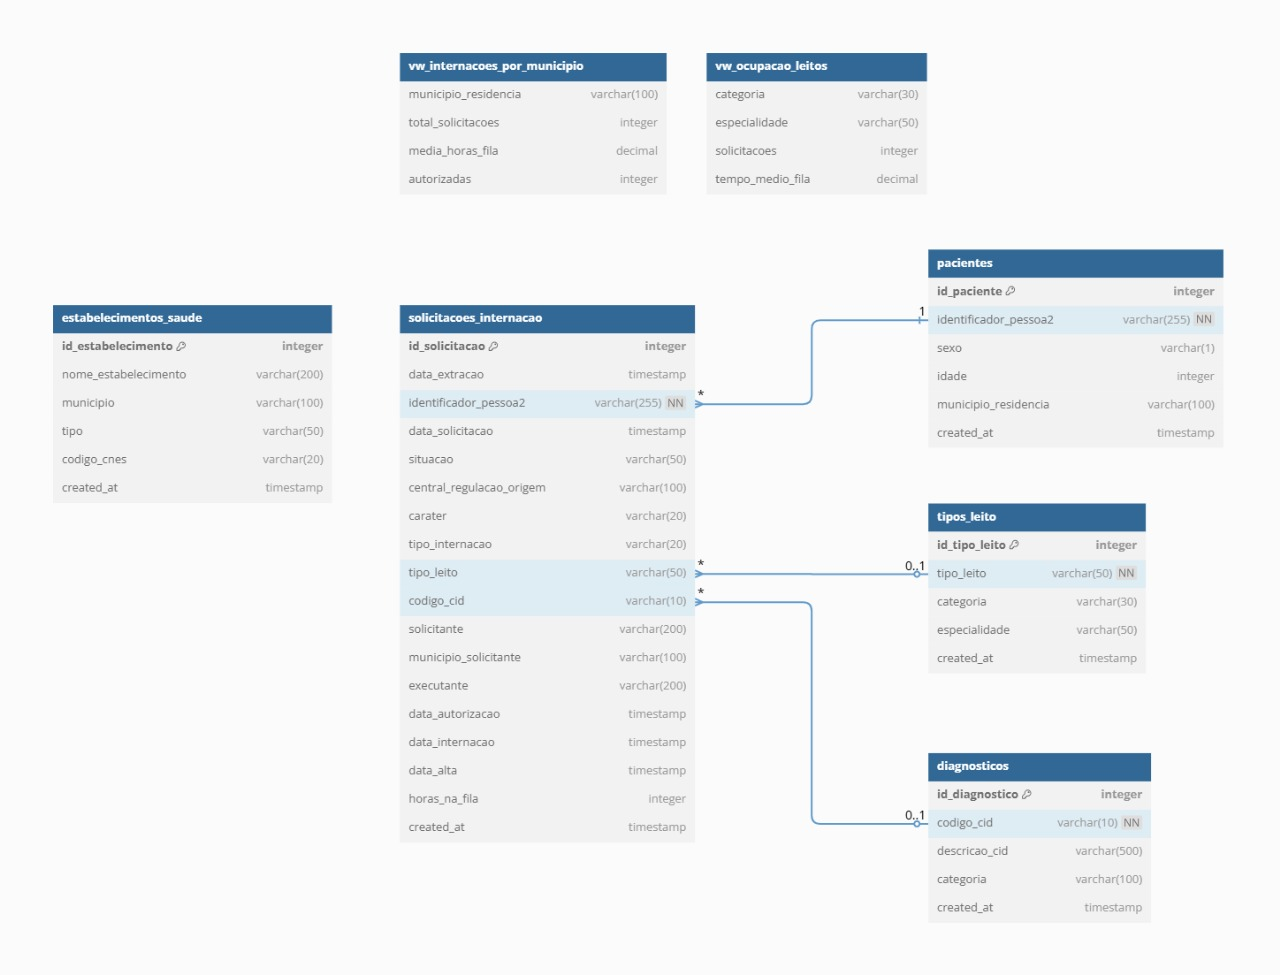
\includegraphics[width=1.0\textwidth]{RELACIONAL_ER_DIAGRAMA.jpg}
\end{center}

\subsection{Script SQL-DDL (Criação das Tabelas) - DBeaver}

\begin{lstlisting}[style=sqlstyle, caption=Criação do Schema e Tabelas]
SET search_path TO gerint;

-- Tabela de Tipos de Leito
CREATE TABLE tipos_leito (
    id_tipo_leito   SERIAL PRIMARY KEY,
    tipo_leito      VARCHAR(50) UNIQUE NOT NULL,
    categoria       VARCHAR(30),
    especialidade   VARCHAR(50),
    created_at      TIMESTAMP DEFAULT CURRENT_TIMESTAMP
);

-- Tabela de Diagnósticos
CREATE TABLE diagnosticos (
    id_diagnostico  SERIAL PRIMARY KEY,
    codigo_cid      VARCHAR(10) UNIQUE NOT NULL,
    descricao_cid   VARCHAR(500),
    categoria       VARCHAR(100),
    created_at      TIMESTAMP DEFAULT CURRENT_TIMESTAMP
);

-- Tabela de Estabelecimentos de Saúde
CREATE TABLE estabelecimentos_saude (
    id_estabelecimento      SERIAL PRIMARY KEY,
    nome_estabelecimento    VARCHAR(200),
    municipio               VARCHAR(100),
    tipo                    VARCHAR(50),
    codigo_cnes             VARCHAR(20),
    created_at              TIMESTAMP DEFAULT CURRENT_TIMESTAMP
);

-- Tabela de Pacientes
CREATE TABLE pacientes (
    id_paciente             SERIAL PRIMARY KEY,
    identificador_pessoa2   VARCHAR(255) UNIQUE NOT NULL,
    sexo                    CHAR(1) CHECK (sexo IN ('M', 'F')),
    idade                   INTEGER CHECK (idade >= 0 AND idade <= 150),
    municipio_residencia    VARCHAR(100),
    created_at              TIMESTAMP DEFAULT CURRENT_TIMESTAMP
);

-- Tabela Principal de Solicitações
CREATE TABLE solicitacoes_internacao (
    id_solicitacao              SERIAL PRIMARY KEY,
    data_extracao               TIMESTAMP,
    identificador_pessoa2       VARCHAR(255) NOT NULL,
    data_solicitacao            TIMESTAMP,
    situacao                    VARCHAR(50),
    central_regulacao_origem    VARCHAR(100),
    carater                     VARCHAR(20) CHECK (carater IN ('Urgência', 'Eletiva', 'Transferência')),
    tipo_internacao             VARCHAR(20) CHECK (tipo_internacao IN ('Própria', 'Não Própria')),
    tipo_leito                  VARCHAR(50),
    codigo_cid                  VARCHAR(10),
    solicitante                 VARCHAR(200),
    municipio_solicitante       VARCHAR(100),
    executante                  VARCHAR(200),
    data_autorizacao            TIMESTAMP,
    data_internacao             TIMESTAMP,
    data_alta                   TIMESTAMP,
    horas_na_fila               INTEGER CHECK (horas_na_fila >= 0),
    created_at                  TIMESTAMP DEFAULT CURRENT_TIMESTAMP,
    
    -- Chaves Estrangeiras
    CONSTRAINT fk_paciente 
        FOREIGN KEY (identificador_pessoa2) 
        REFERENCES pacientes(identificador_pessoa2),
    CONSTRAINT fk_diagnostico 
        FOREIGN KEY (codigo_cid) 
        REFERENCES diagnosticos(codigo_cid),
    CONSTRAINT fk_tipo_leito 
        FOREIGN KEY (tipo_leito) 
        REFERENCES tipos_leito(tipo_leito)
);

-- Indices de Otimizacao
CREATE INDEX idx_solicitacoes_data_solicitacao ON solicitacoes_internacao(data_solicitacao);
CREATE INDEX idx_solicitacoes_municipio ON solicitacoes_internacao(municipio_solicitante);
CREATE INDEX idx_solicitacoes_situacao ON solicitacoes_internacao(situacao);
CREATE INDEX idx_pacientes_municipio ON pacientes(municipio_residencia);
\end{lstlisting}

\subsection{Script SQL-DML (Inserção de Dados - Amostra)}

\begin{lstlisting}[style=sqlstyle, caption=Inserção de Dados de Exemplo]
    -- Insercao de Tipos de Leito
        INSERT INTO tipos_leito (tipo_leito, categoria, especialidade) VALUES
        ('Enfermagem Adulto', 'Enfermaria', 'Adulto'),
        ('Enfermagem Pediatrica', 'Enfermaria', 'Pediatrico'),
        ('Hospital Dia', 'Hospital Dia', 'Geral'),
        ('Obstetrico', 'Enfermaria', 'Obstetrico'),
        ('Psiquiatrico', 'Enfermaria', 'Psiquiatrico'),
        ('UTI Adulto', 'UTI', 'Adulto'),
        ('UTI Neonatal', 'UTI', 'Neonatal'),
        ('UTI Pediatrica', 'UTI', 'Pediatrico'),
        ('UTI Coronariana', 'UTI', 'Cardiologico'),
        ('Bercario', 'Enfermaria', 'Neonatal');

    -- Insercao de Diagnosticos (CID-10)
        INSERT INTO diagnosticos (codigo_cid, descricao_cid, categoria) VALUES
        ('Q90.9', 'Sindrome de Down nao especificada', 'Malformacoes congenitas'),
        ('P07.3', 'Outros recem-nascidos de pre-termo', 'Afeccoes perinatais'),
        ('Q21.9', 'Defeito septal cardiaco congenito nao especificado', 'Malformacoes congenitas'),
        ('P22.0', 'Sindrome do desconforto respiratorio do recem-nascido', 'Afeccoes perinatais'),
        ('Q03.9', 'Hidrocefalia congenita nao especificada', 'Malformacoes congenitas');
\end{lstlisting}

\section{SEGUNDA FONTE DE DADOS - MONGODB}

\subsection{Esquema Lógico NoSQL}

\textbf{Estrutura do Documento de Nascimento:}

\begin{lstlisting}[style=sqlstyle, language=json, caption=Estrutura do Documento MongoDB]
{
  "_id": ObjectId,
  "data_extracao": datetime,
  "data_nascimento": date,
  "peso": int,
  "sexo": "M|F",
  "raca": string,
  "possui_anomalia": "Sim|Nao|Ignorada",
  "cid_anomalia": string,
  "classe_robson": string,
  "local_nascimento": "Hospital|Domicilio|Outro estabelecimento de saude|Outros",
  
  "dados_mae": {
    "escolaridade_mae": string,
    "raca_mae": string,
    "estado_civil_mae": string,
    "nascimento_mae": string,
    "cbo_mae": string,
    "ocupacao": string
  },
  
  "dados_gestacao": {
    "nro_consultas_prenatal": string,
    "cesaria_antes_parto": "Sim|Nao|Nao Sabe|Ignorada",
    "duracao_gestacao": string,
    "gravidez": "Única|Dupla|Tripla"
  },
  
  "dados_parto": {
    "parto": "Vaginal|Cesario|Ignorado",
    "trabalho_parto": "Induzido|Nao induzido|Ignorado",
    "apresentacao_crianca": "Cefalica|Pelvica|Podalica|Transversa|Ignorada"
  }
}
\end{lstlisting}

\subsection{Características da Estrutura NoSQL}

\begin{itemize}
    \item \textbf{Flexibilidade:} Documentos podem ter campos opcionais
    \item \textbf{Aninhamento:} Dados relacionados agrupados em subdocumentos
    \item \textbf{Escalabilidade:} Suporte a grandes volumes de dados de nascimento
    \item \textbf{Consultas:} Índices em campos críticos como data\_nascimento e cid\_anomalia
\end{itemize}

\section{INGESTÃO DE DADOS NO DATA LAKE}

\subsection{Pipeline PostgreSQL → Data Lake}

\textbf{Configuração do Pipeline:}
\begin{itemize}
    \item \textbf{Fonte:} Banco PostgreSQL (gerint schema)
    \item \textbf{Destino:} Azure Data Lake Storage Gen2
\end{itemize}

\textbf{Tabelas Extraídas:}
\begin{itemize}
    \item pacientes
    \item solicitacoes\_internacao
    \item tipos\_leito
    \item diagnosticos
    \item estabelecimentos\_saude
\end{itemize}

\subsection{Pipeline MongoDB → Data Lake}

\textbf{Configuração do Pipeline:}
\begin{itemize}
    \item \textbf{Fonte:} Azure Cosmos DB for MongoDB
    \item \textbf{Destino:} Azure Data Lake Storage Gen2
    \item \textbf{Formato:} JSON
\end{itemize}

\textbf{Coleção Extraída:}
\begin{itemize}
    \item nascimentos
\end{itemize}


\begin{itemize}
    \item \textbf{Padronização de datas:} Formato ISO 8601
    \item \textbf{Limpeza de dados:} Remoção de valores nulos críticos
    \item \textbf{Particionamento:} Por ano/mês para otimização de consultas
\end{itemize}

\section{CONSULTAS SQL NO DATA LAKE}

\subsection{Consulta 1: Análise de Solicitações por Município}

\begin{lstlisting}[style=sqlstyle, caption=Ranking de Municípios por Solicitações]
WITH 
pacientes AS (
    SELECT *
    FROM OPENROWSET(
        BULK 'https://datalakesysteminfra.dfs.core.windows.net/datalakefiles/gerint.pacientes.txt',
        FORMAT = 'CSV',
        FIELDTERMINATOR = ';',
        ROWTERMINATOR = '\n',
        FIRSTROW = 2
    ) WITH (
        id_paciente INT,
        identificador_pessoa2 VARCHAR(255),
        sexo CHAR(1),
        idade INT,
        municipio_residencia VARCHAR(100),
        created_at DATETIME
    ) AS p
),
tipos_leito AS (
    SELECT *
    FROM OPENROWSET(
        BULK 'https://datalakesysteminfra.dfs.core.windows.net/datalakefiles/gerint.tipos_leito.txt',
        FORMAT = 'CSV',
        FIELDTERMINATOR = ';',
        ROWTERMINATOR = '\n',
        FIRSTROW = 2
    ) WITH (
        id_tipo_leito INT,
        tipo_leito VARCHAR(50),
        categoria VARCHAR(30),
        especialidade VARCHAR(50),
        created_at DATETIME
    ) AS tl
),
solicitacoes AS (
    SELECT *
    FROM OPENROWSET(
        BULK 'https://datalakesysteminfra.dfs.core.windows.net/datalakefiles/gerint.solicitacoes_internacao.txt',
        FORMAT = 'CSV',
        FIELDTERMINATOR = ';',
        ROWTERMINATOR = '\n',
        FIRSTROW = 2
    ) WITH (
        id_solicitacao INT,
        data_extracao DATETIME,
        identificador_pessoa2 VARCHAR(255),
        data_solicitacao DATETIME,
        situacao VARCHAR(50),
        central_regulacao_origem VARCHAR(100),
        carater VARCHAR(20),
        tipo_internacao VARCHAR(20),
        tipo_leito VARCHAR(50),
        codigo_cid VARCHAR(10),
        solicitante VARCHAR(200),
        municipio_solicitante VARCHAR(100),
        executante VARCHAR(200),
        data_autorizacao DATETIME,
        data_internacao DATETIME,
        data_alta DATETIME,
        horas_na_fila INT,
        created_at DATETIME
    ) AS s
),
ranking_municipios AS (
    SELECT 
        p.municipio_residencia,
        COUNT(*) AS total_solicitacoes,
        ROUND(AVG(s.horas_na_fila), 2) AS media_horas_fila,
        ROUND(AVG(p.idade), 1) AS idade_media_pacientes,
        MIN(p.idade) AS menor_idade,
        MAX(p.idade) AS maior_idade,
        COUNT(CASE WHEN s.carater = 'Urgência' THEN 1 END) AS urgencias,
        COUNT(CASE WHEN tl.categoria = 'UTI' THEN 1 END) AS solicitacoes_uti
    FROM solicitacoes s
    JOIN pacientes p ON s.identificador_pessoa2 = p.identificador_pessoa2
    JOIN tipos_leito tl ON s.tipo_leito = tl.tipo_leito
    WHERE s.data_solicitacao >= DATEADD(month, -12, GETDATE())
    GROUP BY p.municipio_residencia
    HAVING COUNT(*) >= 10
),
percentis AS (
    SELECT DISTINCT
        PERCENTILE_CONT(0.75) WITHIN GROUP (ORDER BY total_solicitacoes) OVER () AS p75_solicitacoes,
        PERCENTILE_CONT(0.50) WITHIN GROUP (ORDER BY media_horas_fila) OVER () AS mediana_tempo_fila
    FROM ranking_municipios
)
SELECT 
    rm.municipio_residencia,
    rm.total_solicitacoes,
    rm.media_horas_fila,
    rm.idade_media_pacientes,
    rm.menor_idade,
    rm.maior_idade,
    rm.urgencias,
    CASE 
        WHEN rm.total_solicitacoes > p.p75_solicitacoes THEN 'Alta Demanda'
        WHEN rm.total_solicitacoes > p.p75_solicitacoes * 0.5 THEN 'Média Demanda'
        ELSE 'Baixa Demanda'
    END AS classificacao_demanda,
    CASE 
        WHEN rm.media_horas_fila > p.mediana_tempo_fila * 1.5 THEN 'Tempo Crítico'
        WHEN rm.media_horas_fila > p.mediana_tempo_fila THEN 'Tempo Alto'
        ELSE 'Tempo Normal'
    END AS classificacao_tempo_espera
FROM ranking_municipios rm
CROSS JOIN percentis p
ORDER BY rm.total_solicitacoes DESC, rm.media_horas_fila DESC;
\end{lstlisting}

\textbf{Resultado (Primeiras 10 linhas):\\}
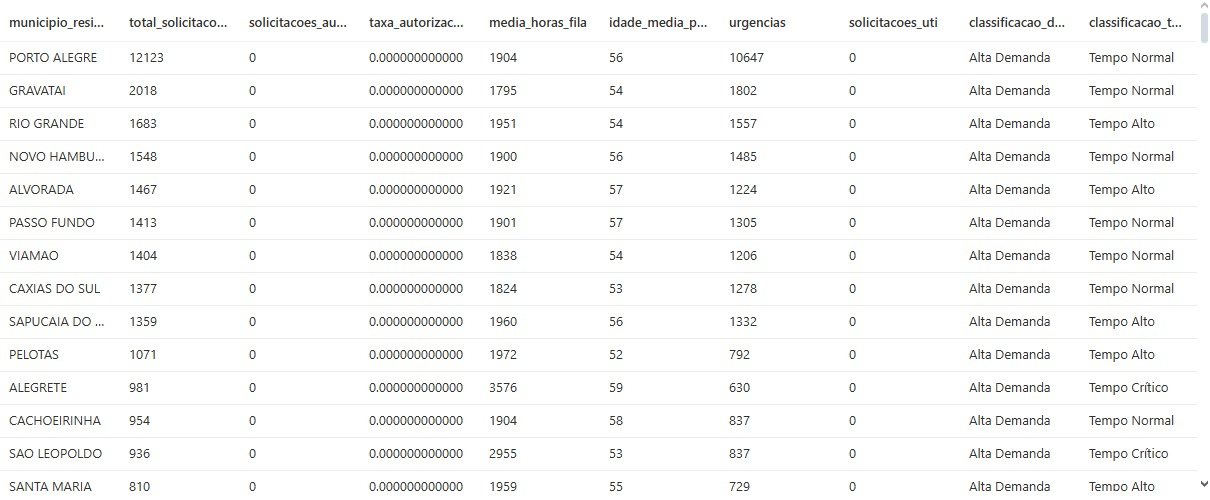
\includegraphics[width=1.0\textwidth]{comnsulta1_result.jpg}

\subsection{Consulta 2: Análise de Especialidades}

\begin{lstlisting}[style=sqlstyle, caption=Análise Por Especialidade]
WITH 
tipos_leito AS (
    SELECT *
    FROM OPENROWSET(
        BULK 'https://datalakesysteminfra.dfs.core.windows.net/datalakefiles/gerint.tipos_leito.txt',
        FORMAT = 'CSV',
        FIELDTERMINATOR = ';',
        ROWTERMINATOR = '\n',
        FIRSTROW = 2
    ) WITH (
        id_tipo_leito INT,
        tipo_leito VARCHAR(50),
        categoria VARCHAR(30),
        especialidade VARCHAR(50),
        created_at DATETIME
    ) AS tl
),
solicitacoes AS (
    SELECT *
    FROM OPENROWSET(
        BULK 'https://datalakesysteminfra.dfs.core.windows.net/datalakefiles/gerint.solicitacoes_internacao.txt',
        FORMAT = 'CSV',
        FIELDTERMINATOR = ';',
        ROWTERMINATOR = '\n',
        FIRSTROW = 2
    ) WITH (
        id_solicitacao INT,
        data_extracao DATETIME,
        identificador_pessoa2 VARCHAR(255),
        data_solicitacao DATETIME,
        situacao VARCHAR(50),
        central_regulacao_origem VARCHAR(100),
        carater VARCHAR(20),
        tipo_internacao VARCHAR(20),
        tipo_leito VARCHAR(50),
        codigo_cid VARCHAR(10),
        solicitante VARCHAR(200),
        municipio_solicitante VARCHAR(100),
        executante VARCHAR(200),
        data_autorizacao DATETIME,
        data_internacao DATETIME,
        data_alta DATETIME,
        horas_na_fila INT,
        created_at DATETIME
    ) AS s
)
SELECT 
    tl.categoria,
    tl.especialidade,
    COUNT(*) AS total_solicitacoes,
    ROUND(AVG(s.horas_na_fila), 2) AS media_tempo_fila,
    COUNT(CASE WHEN s.situacao = 'Autorizada' THEN 1 END) AS autorizadas,
    ROUND(COUNT(CASE WHEN s.situacao = 'Autorizada' THEN 1 END) * 100.0 / COUNT(*), 2) AS taxa_autorizacao
FROM solicitacoes s
JOIN tipos_leito tl ON s.tipo_leito = tl.tipo_leito
WHERE s.data_solicitacao >= DATEADD(month, -6, GETDATE())
GROUP BY tl.categoria, tl.especialidade
ORDER BY total_solicitacoes DESC;
\end{lstlisting}

\textbf{Resultado:\\}
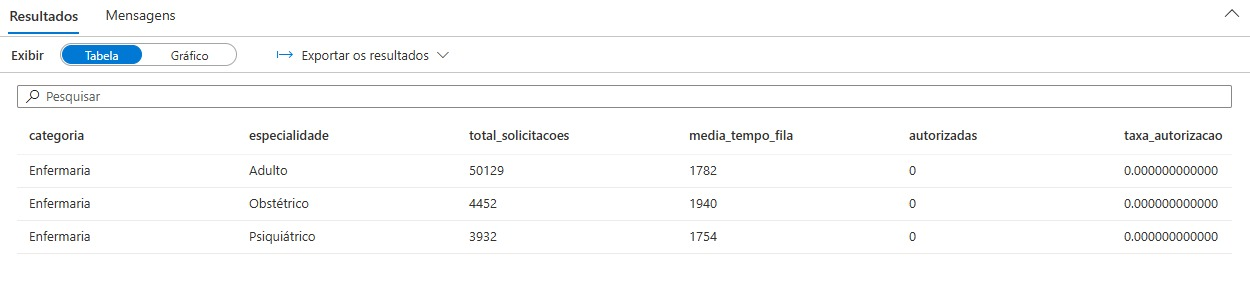
\includegraphics[width=1.0\textwidth]{comnsulta2_result.jpg}
\caption{Distribuição de Especialidades}

\subsection{Consulta 3: Urgências e Não Urgências}

\begin{lstlisting}[style=sqlstyle, caption=Urgências e Não Urgências]
WITH 
solicitacoes AS (
    SELECT *
    FROM OPENROWSET(
        BULK 'https://datalakesysteminfra.dfs.core.windows.net/datalakefiles/gerint.solicitacoes_internacao.txt',
        FORMAT = 'CSV',
        FIELDTERMINATOR = ';',
        ROWTERMINATOR = '\n',
        FIRSTROW = 2
    ) WITH (
        id_solicitacao INT,
        data_extracao DATETIME,
        identificador_pessoa2 VARCHAR(255),
        data_solicitacao DATETIME,
        situacao VARCHAR(50),
        central_regulacao_origem VARCHAR(100),
        carater VARCHAR(20),
        tipo_internacao VARCHAR(20),
        tipo_leito VARCHAR(50),
        codigo_cid VARCHAR(10),
        solicitante VARCHAR(200),
        municipio_solicitante VARCHAR(100),
        executante VARCHAR(200),
        data_autorizacao DATETIME,
        data_internacao DATETIME,
        data_alta DATETIME,
        horas_na_fila INT,
        created_at DATETIME
    ) AS s
),
pacientes AS (
    SELECT *
    FROM OPENROWSET(
        BULK 'https://datalakesysteminfra.dfs.core.windows.net/datalakefiles/gerint.pacientes.txt',
        FORMAT = 'CSV',
        FIELDTERMINATOR = ';',
        ROWTERMINATOR = '\n',
        FIRSTROW = 2
    ) WITH (
        id_paciente INT,
        identificador_pessoa2 VARCHAR(255),
        sexo VARCHAR(20),
        idade INT,
        municipio_residencia VARCHAR(100),
        created_at DATETIME
    ) AS p
),
resultado AS (
    SELECT 
        p.municipio_residencia,
        COUNT(*) AS total_solicitacoes,
        ROUND(AVG(CAST(p.idade AS FLOAT)), 1) AS idade_media,
        COUNT(CASE WHEN s.carater = 'Urgência' THEN 1 END) AS total_urgencias,
        COUNT(CASE WHEN s.carater != 'Urgência' THEN 1 END) AS total_nao_urgencias
    FROM solicitacoes s
    JOIN pacientes p ON s.identificador_pessoa2 = p.identificador_pessoa2
    GROUP BY p.municipio_residencia
)
SELECT TOP 20 *
FROM resultado
ORDER BY total_solicitacoes DESC;

\end{lstlisting}

\section{CONSIDERAÇÕES TÉCNICAS}

\subsection{Arquitetura Implementada}

\begin{itemize}
    \item \textbf{Ingestão:} Azure Data Factory para ETL
    \item \textbf{Armazenamento:} Azure Data Lake Storage Gen2
    \item \textbf{Processamento:} Azure Synapse Analytics
    \item \textbf{Consultas:} SQL Pool e Spark Pool
    \item \textbf{Monitoramento:} Azure Monitor e Log Analytics
\end{itemize}

\subsection{Benefícios Alcançados}

\begin{itemize}
    \item \textbf{Integração:} Visão unificada de dados de saúde
    \item \textbf{Escalabilidade:} Suporte a crescimento de dados
    \item \textbf{Performance:} Consultas otimizadas com particionamento
    \item \textbf{Flexibilidade:} Suporte a dados estruturados e semi-estruturados
\end{itemize}

\section{CONCLUSÃO}

O Data Lake implementado demonstra a viabilidade de integrar diferentes fontes de dados de saúde pública, permitindo análises epidemiológicas avançadas e suporte à tomada de decisão. A correlação entre dados de nascimentos e internações revela padrões importantes para o planejamento da rede de saúde materno-infantil.

A quarta consulta que relaciona diretamente o Relacional ao Não-Relacional está disponível no Synapse como Script6. Optamos por não colar aqui por conta do tamanho da consulta que excede 300 linhas, por conta do formato na qual utilizamos o ROWSET.

Conclui-se que a arquitetura Azure proposta oferece robustez, escalabilidade e flexibilidade necessárias para um sistema de informações de saúde, atendendo aos requisitos técnicos e funcionais estabelecidos.

\vspace{1cm}

\textbf{Fontes de Dados:}
\begin{itemize}
    \item Sistema GERINT - Gestão de Regulação de Internações
    \item SINASC - Sistema de Informações sobre Nascidos Vivos (adaptado)
\end{itemize}

\textbf{Tecnologias Utilizadas:}
\begin{itemize}
    \item Azure Data Lake Storage Gen2
    \item Azure Synapse Analytics  
    \item Azure Database for PostgreSQL
    \item Azure Cosmos DB for MongoDB
    \item Python 3.12 - Pandas (análise e dataload)
\end{itemize}

\end{document}